\section{Verwaltungskontext}

Unter Verwaltungskontext versteht man den Bereich, in welchem sich die öffentlichen Verwaltungen befinden. Die Verwaltung in der Schweiz unterteilt sich in drei Ebenen. Die nationale Ebene, die kantonale Ebene, bestehend aus 26 Kantonen und die Gemeindeebene, bestehend aus ungefähr 2200 Gemeinden \parencite[S. 26-30]{HANDBOEFFVER}.

Die Aufgaben und Kompetenzen der jeweiligen Ebene sind in der Tabelle \ref{tab:aufgabenverwaltungsk} beschreiben. 
\newpage
\begin{table}[h]
	\centering
\begin{tabular}{|p{2.5cm}|p{11.5cm}|}
  \hline
  \textbf{Ebene} & \textbf{Kompetenzen} \\ \hline
   National & Auslandsbeziehungen, Sicherheit, Landesverteidigung, Zivilschutz, Bildung, Forschung, Kultur, Umwelt- und Raumplanung, Öffentliche Arbeiten, Transport, Energie, Kommunikation, die Wirtschaft, Wohnen, Beschäftigung, soziale Sicherheit, Gesundheit, Vorübergehender und ständiger Aufenthalt von Ausländern, das Finanzsystem, Zivilrecht und Strafrecht \\ \hline
   Kantonal & Umweltschutz, Schutz der Natur und des kulturellen Erbes, Regional- / Landnutzungsplanung, Bauvorschriften, Transport und Strassen,Wasser- und Energieversorgung, Abwasserbehandlung und Abfallentsorgung, Aufrechterhaltung der öffentlichen Ordnung und Sicherheit, Sozialhilfe, Arbeit, Behausungen, Gesundheitsvorsorge, Schulen Universitäten und Fachhochschulen, Medien, Kultur, Freizeit, Sport und Erholung, Land-und Forstwirtschaft, Kantonale Nutzungsrechte (für Salz, Wasser, Berge, Jagd und Fischerei), Kantonalbank\\ \hline
   Gemeinde & Kindergarten, Grundschule und Mittelschule, Wohlfahrt, ambulante Pflege, Altenpflege und Sozialversicherungsaufgaben, Abwasser, Müll, Strom, öffentliche Verkehrsmittel innerhalb der Gemeinde, Gemeindezonen- und Landnutzungsplanung, Bauinspektion, Erhaltung des Natur- und Kulturerbes, Strassen und Wege, Sportinfrastruktur und kulturelle Einrichtungen, Ernennung oder Wahl von Beamten, Organisation der Verwaltung und Personalverwaltung, Budgetierung und Buchhaltung, Verwaltung des Eigentums und des Vermögens der Gemeinde und Festlegung des Steuersatzes der Gemeinde, Brandschutzbehörden, Verkehrspolizei und Arbeitsaufsichtsbeamte, Gewährung der Gemeinschaftsbürgerschaft an ausländische Einwohner \\ \hline
  \end{tabular} 
	\caption{Aufgaben und Kompetenzen im Verwaltungskontext \parencite[S. 26-30]{HANDBOEFFVER}}
	\label{tab:aufgabenverwaltungsk}
\end{table}


Alle Organe die zur Erfüllung dieser Aufgaben und Kompetenzen dienen, gelten zum Umfang des Verwaltungskontexts.

Der Einsatz von Webanalysetools im Verwaltungskontext unterscheidet sich von der Privatwirtschaft nicht nur durch die Ziele welche mit den jeweiligen Diensten erreicht werden sollen. Während privatwirtschaftliche Webseiten meistens einem Geschäft dienen, können Webseiten im Verwaltungskontext rein unterstützend sein. Gemäss Umfrage (siehe Anhang \ref{appendix:umfrage}), nutzen die meisten Verwaltung ihren Webauftritt um Informationen anzubieten oder an andere Dienste weiterzuleiten. Vereinzelt werden auch E-Services, wie zum Beispiel online Schalter, angeboten. Verwaltungen unterliegen zudem, aufgrund der kantonalen Datenschutzgesetzen, strengeren Richtlinien was das Auswählen und Einsetzen von Analysetools anbelangt. Da Webanalysetools meist externe Dienste sind, hat man als Anwender dieser Tools oft keinen Einfluss auf die Datenhoheit. Dies bedeutet, dass Einschränkungen durch kantonale Datenschutzgesetze einen Einfluss auf die Auswahlmöglichkeiten von Analysetools haben.

\subsection{Webanalysetools und Datenschutz}
Da das Einsetzen von Webanalyse Tools unumgänglich das Sammeln von Benutzerdaten bedeutet, ist die Handhabung und das Schützen dieser Daten in der Verantwortung jeder Organisation, die Webanalyse betreibt. Mit zunehmender Wichtigkeit der Webanalyse und dem technischen Fortschritt, können die Analysen nun immer genauer ausfallen. Mittlerweile kann bis zur Mausbewegung herunter das Verhalten des Benutzers einer Webseite aufgezeichnet werden \parencite[S. 1]{EcommerceUndDatenschutz}. Dies kann, wenn nicht sorgfältig mit den Daten umgegangen wird, Verletzungen des Datenschutzrechtes zur Folge haben.

Webanalysetools sind in der Lage, die Benutzerinteraktionen feingranular aufzuzeichnen. Dies geschieht mittels Cross-Domain-Tracking sogar über mehrere Webseiten hinweg. Die zusammengeführten Daten können und werden von einigen Webanalysetools eindeutigen Benutzern zugeordnet. Hierbei spricht man von einer personalisierten Webanalyse, bei welcher Nutzerprofile erstellt werden und Zielgruppenanalysen durchgeführt werden. Diese Art von Webanalyse gilt generell gesehen aus Datenschutzgründen als problematisch \parencite[S. 2]{EcommerceUndDatenschutz}. Gemäss Bundesgesetz \parencite[§§ 4 Abs. 5]{SDSG} gilt im Allgemeinen, dass Personendaten nur gesammelt und bearbeitet werden dürfen, sofern eine explizite Einwilligung durch die betroffenen Person besteht. Die Einwilligung ist nur gültig, wenn diese freiwillig und nach angemessener Informationen erfolgt. Hinzu kommt, dass gemäss dem Schweizer Bundesgesetz \parencite[§§ 6 Abs. 1]{SDSG} Personendaten nur im Ausnahmefall ins Ausland weitergegeben werden dürfen. Dies ist bei Webanalysetools, welche die Daten auf Servern im Ausland verarbeiten, problematisch.

Webanalysen können aber auch aufgrund von anonymisierten, respektive pseudonymisierten Daten durchgeführt werden. Bei pseudonymisierten Daten sind lediglich die Identifikationsmerkmale wie Name und Adresse durch Kennzeichen ausgetauscht, um Rückschlüsse zu erschweren. Von einer Anonymisierung spricht man, sofern die personenbezogenen Daten so verändert wurden, dass die Daten nicht mehr einer natürlichen Person zugeordnet werden können \parencite[S. 3]{EcommerceUndDatenschutz}. Dies bedeutet unter anderem, dass es sich bei den gesammelten Daten lediglich um Metriken handelt, welche keine Person eindeutig identifizierbar machen. Dazu gehören Metadaten wie zum Beispiel Name, Adresse oder E-Mail-Adresse. Auch IP-Adressen, welche üblicherweise von Analysetools zur Geolokalisierung verwendet werden, gelten als personenbezogene Daten. Dies fordert Webanalysten, welche durch anonymisierung der Daten den Datenschutz gewährleisten, dazu auf die IP-Adressen so zu kürzen, dass nicht mehr auf die Person rückgeschlossen werden kann.\parencite[S. 4]{EcommerceUndDatenschutz}.

Trotz allen Vorkehrungen die getroffen werden, um den Datenschutz zu gewährleisten, erfordert ein rechtskonformer Einsatz von Analysetools auch in Zukunft eine genaue Analyse der Rechtslage und kann nicht pauschal das eine oder das andere Tool richtig geheissen werden \parencite[S. 6]{EcommerceUndDatenschutz}.

\subsection{Das kantonale Datenschutzgesetz}
Zusätzlich zum Bundesgesetz für Datenschutz unterliegen Verwaltungen dem jeweiligen kantonalen Datenschutzgesetz. Die kantonalen Datenschutzgesetze regeln die Rechtslage zum Schützen von Personen vor Datenmissbrauch durch die Behörden \parencite[Vgl. §§ 1 Abs. 1]{DSSGBERN}. 

Die strikten und von Kanton zu Kanton unterschiedlichen Gesetze zum Datenschutz, erschweren eine rechtskonforme Webanalyse. Das Erheben von Personendaten, welche nicht anonymisierten werden, steht im Konflikt mit mehreren kantonalen Datenschutzgesetzen \parencite[Vgl. §§ 15 Abs. 1]{DSSGBERN}. Falls die Daten nicht ausreichend anonymisiert werden, gibt es durch diverse Gesetzesartikel, wie zum Beispiel Artikel 7 des kantonalen Datenschutzgesetzes des Kanton Glarus \parencite[§§ 7 Abs. 1]{DSSGGL}, welcher vorschreibt die Datenbeschaffung für betroffene Personen in erkennbarer Weise durchzuführen, Schwierigkeiten. Kaum ein Webanalysetool vermag es, die gesetzlichen Vorschriften einzuhalten, sollten nicht anonymisierte Daten verwendet werden.

In der unten stehenden Tabelle \ref{tab: ktrechtslage} ist veranschaulicht, welche Gesetzesartikel die Handhabung anonymisierter Daten regeln und wie die Rechtslage im jeweiligen Kanton aussieht.

\begin{longtable}{| p{.20\textwidth} | p{.75\textwidth}|} 
		\hline
		\textbf{Kanton} & \textbf{Rechtslage}  \\ 
    \hline
    Aargau & Im Kanton Aargau ist das Verwenden von Personendaten für nicht personenbezogene Zwecke (Forschung, Planung und Statistik) erlaubt, wenn Personendaten anonymisiert werden, Empfänger der Personendaten diese nur mit Zustimmung des öffentlichen Organs weitergibt und betroffene Personen bei der Veröffentlichung nicht erkennbar sind \parencite[§§ 19 Abs. 1]{DSSGAARGAU}. \\
    \hline
		Appenzell Ausserrhoden & Das kantonale Datenschutzgesetz erlaubt die Bearbeitung von personenbezogenen Daten für nicht personenbezogene Zwecke, namentlich für Statistik, Planung und Forschung, wenn die Daten anonymisiert werden und die Ergebnisse der Bearbeitung keine Rückschlüsse auf betroffene Personen erlauben \parencite[§§ 14 Abs. 1]{DSSGAARh}. \\
    \hline
		Appenzell Innerrhoden & In Appenzell Innerrhoden dürfen Personendaten für nicht personenbezogene Zwecke bearbeitet werden, wenn sie anonymisiert sind und das Ergebnis keine Rückschlüsse auf betroffene Personen erlaubt. Personendaten dürfen Privaten überlassen werden, sofern die Bestimmung und Geheimhaltung gewährleistet sind \parencite[§§ 7 Abs 1-2]{DSSGAIRh}.\\
    \hline
		Basel-Landschaft & Das kantonale Datenschutzgesetz des Kanton Basel-Landschaft erlaubt das Verarbeiten von Personendaten zu einem nicht personenbezogenen Zweck, wenn die Daten so anonymisiert werden, dass keine Rückschlüsse auf die betroffenen Personen möglich sind \parencite[§§ 11 Abs. 2]{DSSGBL}. Wenn die betroffene Person im Einzelfall einwilligt, dürfen die Personendaten zu ausschliesslich dem Zweck verwendet werden, zu dem sie erhoben worden sind \parencite[§§ 11 Abs. 1]{DSSGBL}. \\
		\hline
		Basel-Stadt &  Gemäss Datenschutzgesetz des Kanton Basel-Stadt \parencite[§§ 10 Abs. 1]{DSSGBS} dürfen Personendaten für nicht personenbezogene Zwecke (Statistik, Planung, Wissenschaft und Forschung) verwendet werden, wenn die Daten nicht für einen personenbezogenen Zweck weitergegeben werden, die Daten anonymisierten oder pseudonymisiert werden und die Ergebnisse so bekannt gegeben werden, dass keine Rückschlüsse auf betroffene Personen möglich sind. \\
		\hline
    Bern & Der Kanton Bern erlaubt gemäss \parencite[§§ 15 Abs. 1]{DSSGBERN} das Bearbeiten der Daten für Forschung, Praxisbildung, Statistik oder Planung, sofern die Daten anonymisierten oder ohne direkte Personenkennzeichnung verwendet werden. \\
		\hline
		Freiburg & Das Freiburger Datenschutzgesetz erlaubt das Einholen von Personendaten durch öffentliche Organe für nicht personenbezogene Zwecke \parencite[§§ 14 Abs. 1]{DSSGFR}. Die Personendaten müssen anonymisiert werden oder ohne direkten Bezug auf betroffene Personen verwendet werden. Ergebnisse müssen so veröffentlicht werden, dass die betroffenen Personen nicht bestimmbar sind \parencite[§ 16 Abs. 1-2]{DSSGFR}.  \\
		\hline
    Genf & Personendaten dürfen zur Verarbeitung an Dritte weitergegeben werden, sofern dies nicht durch die Geheimhaltungspflicht verboten ist, der Unterauftrag der Verarbeitung Gegenstand eines rechtlichen Vertrages ist und bei Verarbeitung im Ausland der Empfängerstaat ein angemessenes Schutzniveau gewährleistet \parencite[§§ 13A Abs. 1-5]{DSSGGE}. \\
		\hline
		Glarus & Laut kantonalem Datenschutzgesetz ist es erlaubt öffentlichen Organen erlaubt Personendaten zu nicht personenbezogenen Zwecken zu bearbeiten, falls Daten anonymisiert werden und die Ergebnisse so veröffentlicht werden, dass Betroffene nicht bestimmbar sind. Es gelten ausserdem besondere Vorschriften für den Bereich der medizinischen Forschung \parencite[§§ 11 Abs 1-2]{DSSGGL}. \\
		\hline
		Graubünden & Es gelten die Definitionen gemäss Bundesgesetz \parencite[§§ 2 Abs. 2-3]{DSSGGR}.  \\
		\hline
		Jura & Kanton Jura teilt sich das Datenschutzgesetz mit dem Kanton Neuenburg \parencite[S. 1 Abs. 2]{JURAAbkommenNE}. \\
		\hline
		Neuenburg & Öffentliche Organe des Kanton Neuenburg haben die Erlaubnis Personendaten zu nicht personenbezogenen Zwecken zu verwenden, sofern diese anonymisiert werden, die Weitergabe an dritte durch Zustimmung der Behörde geschieht, und keine betroffenen Personen aus den Ergebnissen auslesbar sind \parencite[§§ 25 Abs. 1]{DSSGNE}. \\
		\hline
		Nidwalden & Personendaten dürfen zu nicht personenbezogenen Zwecken bearbeitet werden, wenn die Daten anonymisiert werden, Daten nur mit Zustimmung des Organs an dritte weitergegeben werden und aus den Ergebnissen betroffene Person nicht bestimmbar sind \parencite[§§ 16 Abs 1-2]{DSSGNW}. \\
		\hline
		Obwalden & Es gilt das Bundesgesetz \parencite{DSSGOW} \\
		\hline
		Schaffhausen & Organe des Kanton Schaffhausen dürfen Personendaten für nicht personenbezogenen Zwecke verwenden, wenn die Daten anonymisierten werden, Ergebnisse keine Bestimmung betroffener Personen zulässt und die Zustimmung des Datenschutzbeauftragten vorliegt \parencite[§§ 12 Abs. 1]{DSSGSH}. Personendaten dürfen an private Personen oder Organisationen bekannt gegeben werden, wenn diese nicht an dritte weitergegeben werden und für die Datensicherheit gesorgt ist. Bei der Weitergabe ist eine Vereinbarung abzuschliessen \parencite[§§ 12 Abs 2]{DSSGSH} \\
		\hline
    Schwyz & Es dürfen Personendaten für nicht personenbezogene Zwecke bearbeitet werden, wenn die Daten anonymisiert werden und die Ergebnisse keine betroffenen Personen bestimmbar machen. Die Daten dürfen weitergegeben werden, wenn der Empfänger sich dazu verpflichtet, die Daten nicht an Dritte weiterzugeben. \parencite[§§ 14 Abs 1-2]{DSSGSZ} \\

		\hline
		Solothurn & Das Bearbeiten von Personendaten zu nicht personenbezogenen Zwecken ist erlaubt, wenn die Daten anonymisiert werden \parencite[§§ 16 Abs 3]{DSSGSO}. \\
    \hline
		St. Gallen & Das öffentliche Organ muss Personendaten, die es für einen nicht personenbezogenen Zweck verwendet Anonymisieren. Es muss sichergestellt werden, dass aus den Ergebnissen keine Rückschlüsse auf Betroffene möglich sind. Bei der Weitergabe muss durch den Empfänger eine schriftliche Verpflichtung vorliegen, die Daten nicht weiterzugeben und die generell geltenden Gesetze einzuhalten\parencite[§§ 7 Abs 1-3]{DSSGSG}. \\
		\hline
		Tessin & Organe des Kanton Tessin dürfen Personendaten für nicht personenbezogene Zwecke bearbeiten, wenn die Daten anonymisiert werden, der Empfänger die Daten mit Genehmigung der zuständigen Stelle erhalten hat, die Ergebnisse so veröffentlicht werden, dass keine Rückschlüsse auf betroffene Personen möglich sind und der Empfänger der Daten die Bestimmungen der Geheimhaltung einhält \parencite[§§ 15 Abs 1-2]{DSSGTI}. \\
		\hline
		Thurgau & Personendaten für nicht personenbezogene Zwecke dürfen bearbeitet werden, wenn diese anonymisiert werden, sodass keine Rückschlüsse auf Betroffene möglich sind. Die Personendaten dürfen weitergegeben werden, falls der Empfänger die Daten nicht an dritte weiter gibt und für die Datensicherheit gesorgt ist \parencite[§§ 11 Abs 1-3]{DSSGTG}. \\
		\hline
		Uri & Für Forschung, Planung und Statistik ist es erlaubt Personendaten für nicht personenbezogene Zwecke zu bearbeiten. Dabei sind die Daten zu anonymisieren, sodass bei der Veröffentlichung der Ergebnisse betroffene Person nicht bestimmbar sind. Wenn keine besonderen Geheimhaltungsbestimmungen bestehen, können die Personendaten an andere Behörden zur Bearbeitung weitergegeben werden \parencite[§§ 10 Abs. 1-2]{DSSGUR}. \\
		\hline
    Waadt & Das Bearbeiten von Personendaten zu nicht personenbezogenen Zwecken ist gestattet, wenn die Daten anonymisiert werden, es aus den Ergebnissen keine Rückschlüsse auf betroffene Personen möglich sind, die Daten, falls sie weitergegeben werden, nicht an Dritte übertragen werden \parencite[§§ 24 Abs 1-3]{DSSGVD}. \\
		\hline
    Wallis & Für Zwecke der Wissenschaft, der Statistik, der Planung oder Forschung dürfen Personendaten zu nicht personenbezogenen Zwecken bearbeitet werden, falls Resultate keine Rückschlüsse auf Betroffene ermöglichen \parencite[§§ 26 Abs. 1]{DSSGVS}.  \\
		\hline
    Zug & Daten dürfen für Forschung, Planung und Statistik bearbeitet werden, wenn sie nicht weitergegeben werden, anonymisiert werden und sich aus den Ergebnissen betroffene Personen nicht bestimmen lassen \parencite[§§ 4 Abs 1e]{DSSGZG}. \\
		\hline
    Zürich & Zum Bearbeiten von Personendaten zu nicht personenbezogenen Zwecken, muss der Empfänger nachweisen, dass Personendaten anonymisiert werden und aus den Ergebnissen Rückschlüsse auf die betroffenen Personen unmöglich sind \parencite[§§ 18 Abs. 1-2]{DSSGZH}. \\
		\hline

    \caption{Kantonale Rechtslage}
    \label{tab: ktrechtslage}
	\end{longtable}

  Wie aus der Tabelle \ref{tab: ktrechtslage} entnommen werden kann,
  legt ein Grossteil der Kantone fest, dass für Statistiken Personendaten verwendet werden dürfen, sofern diese anonymisiert sind und aus den Ergebnissen keine Rückschlüsse auf betroffenen Personen möglich sind. In wenigen fällen ist geregelt, dass auch die Weitergabe zur Verarbeitung der anonymisierten Daten eingeschränkt ist. Für die Webanalysetools ist dies ein wichtiger Punkt. Die Verarbeitung der Daten findet bei den meisten Analysetools, die als SaaS oder ASP angeboten werden, auf zentralen Servern im Ausland statt. Nur wenn die Webanalyse In-House betrieben wird, kann davon ausgegangen werden, dass Daten nicht zur Verarbeitung weitergegeben werden \parencite[S 174-176]{nakatani2011toolselectionmethod}.


\subsection{Strategien zur Datenschutzkonformität}
Webanalysetools an sich, sind nicht datenschutzkonform \parencite[S. 1-4]{EcommerceUndDatenschutz}. Es liegt am Webanalysebetreiber, das richtige Tool auszuwählen und in erster Linie das Tool richtig zu Konfigurieren, sodass keine Datenschutzgesetze verletzt werden.

Folgende Strategien gelten als Standard für die Datenschutzkonformität \parencite[S. 2-5]{EcommerceUndDatenschutz}:

\begin{description}
  \item[Anonymisierung] Daten lassen keine Rückschlüsse auf die betroffenen Personen zu. Dazu gehört auch das Kürzen der IP-Adresse, was nicht in machen Analysetools eingestellt werden muss \parencite[S. 3]{EcommerceUndDatenschutz}.
  \item[In-House Datenverarbeitung] Dies ist eine Funktion, welche nicht jedes Tool zur Verfügung stell. Zudem erfordert die In-House-Datenverarbeitung zusätzliches Know-how, da ein Service für die Datenverarbeitung installiert und betrieben werden muss \parencite[S. 175]{nakatani2011toolselectionmethod}. 
  \item[Datenverarbeitungsvertrag mit dem Tracking-Service Provider] Wenn es das Gesetz vorschreibt, das die Weitergabe von Daten vertraglich geregelt werden muss, wird dies von grossen Service Provider wie zum Beispiel Google Analytics angeboten. Google bietet Musterverträge für Auftragsdatenverarbeitung an \parencite[S. 5]{EcommerceUndDatenschutz}. 
  \item[Explizite Einwilligung durch Benutzer] Die Benutzer werden durch diese Massnahme erst getrackt, wenn sie explizit einwilligen. Um rechtlich gültig zu sein, muss die Einwilligung informiert und freiwillig erfolgen. Das explizite Einwilligen kann erfordert oder erbittet werden. Wird es erfordert, kann der Dienst nur verwendet werden, wenn eingewilligt wird. Der Vorteil dieser Methode ist es, dass die Daten die erhoben werden komplett sind. Der Nachteil jedoch, dass einige Benutzer den Dienst meiden werden. Wird die Einwilligung erbittet, kann der Dienst genutzt werden, ohne das Tracking aktiv ist. Hierbei ist der Vorteil, dass durch die Massnahme kein Traffic verloren geht. Der Nachteil wiederum ist, dass sich die Statistik verfälschen wird. \parencite[S. 2-3]{EcommerceUndDatenschutz}.
  \item[Opt-Out] Anders als bei der expliziten Einwilligung, erfordert diese Massnahme aktives Engagement durch den Besucher. Er wird beim Aufrufen der Webseite getrackt und es ist in der Verantwortung des Besuchers das Tracking unterbinden zu lassen. Diese Methode ist aus Datenschutzsicht mangelhaft \parencite[§§ 9 Abs. 4]{DSSGBERN}, kann aber dennoch für Benutzer interessant sein, um sich vor Tracking zu schützen.
\end{description}

\newpage

\section{Webanalysetools}

Firmen, Privatpersonen, Ämter, Politiker, Selbstständige und viele mehr Nutzen das Internet für den Austausch, das Anbieten und auch für das Erlangen von Informationen, das Kaufen und Verkaufen von Gütern, sowie das Austauschen von Nachrichten. Bietet man im Internet einen Dienst an, ist dieser meist zugänglich für die ganze Welt. Nun wäre es für den Anbieter der Informationen interessant, gewisse Dinge über die Abrufe herauszufinden. Wer ruft die Informationen ab? Wie gelangen die User auf meine Seite und wie navigieren sie zu den Informationen die sie Benötigen \parencite[S. 175]{nakatani2011toolselectionmethod}?

Mit genau diesen Fragen beschäftigen sich die Webanalysetools. Sie bieten durch das Messen, Sammeln und Analysieren von Benutzerdaten eine vertiefte Einsicht in die Benutzung des Dienstes und zeigen dadurch Schwachstellen oder Verbesserungspotenzial auf \parencite[S. 1]{waisberg2009webShort}. 
Webanalysetools dienen hauptsächlich zwei Zwecken. Der eine Zweck ist es, den Anbieter des Dienstes dabei unterstützen seine Ziele zu erreichen \parencite[S. 56]{AnalyticsForDummies}. Diese Ziele können sich von Dienst zu Dienst unterscheiden. Bei einem Online-Shop wäre das effektive Ziel die Besucher in Käufer umzuwandeln \parencite[S. 28]{AnalyticsForDummies}. Handelt es sich bei dem Dienst um eine informative Dienstleistung, so könnte ein Ziel des Anbieters sein, den User in einen wiederkehrenden User umzuwandeln, indem man ihn beispielsweise ein Konto erstellen lässt. Abgesehen von Zielen gibt es auch Zwischenziele. Ein Beispiel hierfür wäre das Abonnieren eines Newsletters, durch welchen mit dem User interagiert werden kann. Der zweite Zweck von Webanalysetools ist es, das Erlebnis der Benutzer die mit dem Dienst interagieren besser zu verstehen, damit deren Erlebnis zukünftig verbessert werden kann \parencite[S. 1]{waisberg2009webShort}.

\subsection{Typen von Webanalyse}

Webanalyse lässt sich aufgrund von verschiedenen Charakteristiken Gruppieren \parencite[S. 172-174]{nakatani2011toolselectionmethod}.

\begin{description}
  \item[Methode der Datensammlung] Bezieht sich auf die technische Art wie die Daten gesammelt werden. Dazu gehören: Web Beacon, Packet Sniffing, Transaktionsloganalyse und Page Tagging.  
  \item[Art des Zugriffs auf den Service] Erklärt die Bereitstellung des Aufzeichnungs- und Analyseservices. Dazu zählen: Software as a Service (SaaS), Application Service Provider und In-House.
  \item[Typ des zu verfolgenden Gerätes/Systems] Beinhaltet die Arten der Zielsysteme welche analysiert werden können. Beispiele für solche Systeme sind: Mobilgeräte, Browser oder Nativ-Applikationen.
  \item[Datenverfügbarkeit und Geschwindigkeit] Bezieht sich auf die Unterschiede in der Geschwindigkeit beim Bereitstellen der aufgezeichneten Daten. Einige Tools ermöglichen Analysen in Echtzeit, während andere Minuten bis zu Stunden brauchen, um die Daten aufzubereiten.
\end{description}

Anhand der Gruppierung auf Basis der Methode der Datensammlung lässt sich ein guter Überblick an Tools auf dem Markt schaffen. Die Datensammlung lässt sich im Wesentlichen auf vier verschiedene Arten durchführen, wobei Transaktionsloganalyse und Page Tagging als die am häufigsten eingesetzten Tools gelten. In den letzten Jahren jedoch, gewann die Page Tagging Methode deutlich an Popularität, während Log Analyse immer weniger häufig eingesetzt wird \parencite{nakatani2011toolselectionmethod}.

\subsubsection{Web Beacon} 
Bei Web Beacons handelt es sich um kleine Bilddateien, welche sich auf einer Webseite eingefügt werden können und per Request angefordert werden \parencite[S. 173]{nakatani2011toolselectionmethod}. Web Beacons werden in der Praxis nur noch selten eingesetzt. Sie Werden hauptsächlich dafür verwendet, Kundenverhalten über mehrere Webseiten hinweg zu verfolgen. Eine der häufigsten Applikationen ist das Bewerten der Leistung von Bannerwerbung. Für einfache Webanalyse wird diese Methode eher selten verwendet \parencite[S. 3]{waisberg2009webShort}.

\subsubsection{Packet Sniffing}
Durch das Abfangen und analysieren der Webpakete auf dem Webserver, können mit Packet Sniffing Daten gesammelt werden. Packet Sniffing findet in der Praxis hauptsächlich Anwendung bei multivariatem Testen \parencite[S. 4]{waisberg2009webShort}.

\subsubsection{Transaktionsloganalyse} 
Bei dieser Methode werden die Logdateien auf dem Webserver analysiert. Transaktionsloganalyse ist eine in der Praxis nach wie vor verwendete Methode, um Daten über Webseitenaufrufe zu sammeln.\parencite[S. 173]{nakatani2011toolselectionmethod}. Die Tiefe der Daten, die gesammelt werden können, hält sich jedoch im Vergleich zu anderen Methoden in Grenzen. Es lassen sich durch Transaktionsloganalyse folgende Informationen Sammeln \parencite[S. 2]{waisberg2009webShort}:

\begin{description}
  \item[IP] Die IP-Adresse des Computers, der die Webseite angefordert hat
  \item[Datum und Zeit] Zeitpunkt des Anfordern der Daten
  \item[Verarbeitungszeit] Wie lange die Transaktion gedauert hat
  \item[Grösse] Anzahl Bytes die übertragen wurden
\end{description}

Ausserdem bietet Transaktionsloganalyse gegenüber den anderen Methoden die folgenden Vorteile\parencite[S. 2]{waisberg2009webShort}:

\begin{description}
  \item[Dateneigentum] Der Besitzer der Webseite ist ebenfalls der Besitzer der Logs und somit der gesammelten Daten. 
  \item[Rückwärts Verfügbarkeit] Die Daten in den Logs können, solange sie gespeichert bleiben, erneut analysiert und verarbeitet werden. 
  \item[Speichert Verhalten von Crawler] Da auch Hits von Crawler Transaktionen sind, werden diese in den Logs gespeichert. Sie sind zwar nicht notwendig für die Analyse der menschlichen Aktivitäten, doch sind sie wichtig für die Suchmaschienenoptimierung \parencite[S. 174]{nakatani2011toolselectionmethod}. 
\end{description}


\subsubsection{Page Tagging} 
Page Tagging ist die Sammlung der Daten von Webseitenbesucher durch ein JavaScript-File auf jeder Webseite. Dieses JavaScript-File zeichnet das Verhalten des Seitenbesuchers auf, und sendet die Informationen an einen zentralen Datensammlungsserver \parencite[S. 173]{nakatani2011toolselectionmethod}.

PageTagging ermöglichte es, im Gegensatz zu Transaktionsloganalyse, detaillierter Daten aufzuzeichnen. Da das JavaScript-Programm lokal auf dem Computer des Webseitenbesuchers ausgeführt wird, ist die Art der Daten, die gesammelt werden können, beinahe unbegrenzt. Durch das Modifizieren des JavaScript-Codes kann beliebig angepasst werden, welche Daten das gesammelt werden sollen \parencite[S. 3]{waisberg2009webShort}. 

Ausserdem bietet Page Tagging gegenüber den anderen Methoden die folgenden Vorteile \parencite[S. 174]{nakatani2011toolselectionmethod}:

\begin{description}
  \item[Präzision] Page Tagging zählt alle Hits, die durch Webbrowser ausgeführt werden. Durch das ausführen des JavaScript-Programm werden auch wenn die Seite im Cache ist die Hits gezählt.
  \item[Client-Side Aktivitäten] Durch die Gegebenheit, dass Page Tagging lokal ausgeführt wird, können nebst Seitenaufrufen weitere Daten aufgezeichnet werden.
  \item[Wiederkehrende Besucher] Durch den Einsatz von Cookies kann mittels Page Tagging einfach herausgefunden werden, ob es sich um neue oder wiederkehrende Besucher handelt.
  \item[Outsourcing] Page Tagging wird üblicherweise in Form eines Services angeboten. Organisationen, welche nicht über die Infrastruktur verfügen In-House Analysen durchzuführen sind auf solche Services angewiesen.
\end{description}

Die Umfrage (Anhang \ref{appendix:umfrage}) hat ergeben, dass alle der Befragten, die Webanalyse betreiben, ein Webanalysetool einsetzen, welches die Methode des Page Tagging verwendet. Somit kann gesagt werden, dass Page Tagging heutzutage die populärste Methode ist Webanalyse zu betreiben.

\newpage
\section{Marktangebot der Webanalysetools}\label{sec:marktangebotwebanalyse}
Es gibt eine riesige Menge an Tools, die auf dem Markt verfügbar sind. Gemäss \parencite{datanyzeSwitzerlandWebanalytics}, sind in der Schweiz 129 verschiedene Webanalysetools im Einsatz. Dabei macht Google Analytics mit Abstand den grössten Teil aus. 82.78\% des Marktes verwendet Google Analytics . Mit nur 3.48\% ist Facebook Analytics der zweit grösste Anbieter am Markt. Matomo ist der am Schweizer Markt dritt grösste Anbieter. Matomos Marktanteil beträgt 2.8\%. Hotjars Marktanteil ist 1.2\%, während sich Monster Insights Marktanteil auf 0.9\% beläuft. 

\begin{figure}[h]
  \centering
\begin{tikzpicture}
\pie[] {
82.78/ Google Analytics,
3.48/ Facebook Analytics,
2.78/ Matomo,
1.27/ HotJar,
8.77/ Andere,
0.92/ MonsterInsights
}
\end{tikzpicture}
\caption{Marktanteile der Top-5 Webanalysetools in der Schweiz \parencite{datanyzeSwitzerlandWebanalytics}}
\label{fig:marktanteil}
\end{figure}


Anders als beim kompletten Schweizer Markt, wurden in der Umfrage (siehe Anhang \ref{appendix:umfrage}) lediglich Verwaltungen befragt. Dementsprechend sah die Verteilung der eingesetzten Tools, dargestellt in Abbildung \ref{fig:verwVerteilungTools}, anders aus.

\begin{figure}[h]
  \centering
\begin{tikzpicture}
\pie[] {
39.1/ i-CMS,
4.3/ Google Analytics,
8.7/ CMS integriert,
21.7/ Matomo,
4.3/ Ryte,
8.7/ SiteImprove,
13.2/ keine Angaben}
\end{tikzpicture}
\caption{(N=23) Verwendung von Analysetools in Verwaltungen Gem. Umfrage (Siehe Anhang \ref{appendix:umfrage})}
\label{fig:verwVerteilungTools}
\end{figure}

Den grösste Teil der Befragten, verwendet das von Innovative Web AG in das CMS integrierte Analysetool i-CMS oder Matomo. Vereinzelt werden die Tools Google Analytics, Ryte und SiteImprove verwendet. Auch gibt es Anwender, die angaben, dass sie ein in das CMS integriertes Tool verwenden. Dabei wurden keine Angaben gemacht, um welches CMS-Tool es sich handelt.

In den folgenden abschnitten werden die zwei meist benutzen Analysetools in der Schweiz gemäss Datanyze \parencite{datanyzeSwitzerlandWebanalytics}, sowie die zwei meist genutzten Analysetools der Verwaltungen gemäss Umfrage (siehe Anhang \ref{appendix:umfrage}) genauer analysiert.


\subsection{Google Analytics}\label{subsec:GoogleAnalytics}
Google Analytics ist sowohl in der Schweiz als auch Global das am meisten eingesetzte Webanalyse Tool \parencite{datanyzeSwitzerlandWebanalytics}. 

\subsubsection{Funktionalitäten und Eigenschaften}
Gemäss dem Hersteller und Anbieter des Services Google Analytics, weist das Analysetools folgende Eigenschaften auf:

\begin{table}[h]
	\centering
	\begin{tabular}{ | p{4cm} | p{10cm} |}
		\hline
		\textbf{Kriterium} & \textbf{Eigenschaft}  \\ 
		\hline
		Preis & Gratis \\
    \hline
    On-Premise / In-House & Nein \\
    \hline
    Datenaktualität & weniger als 24 Stunden \\
    \hline
    Datenvolumen & 10'000'000 Hits pro Monat\\
    \hline
    Maximale Anzahl Metriken / Dimensionen & 20\\
    \hline
    Datenerfassung und -Verwaltung &  Page Tagging, API für externe Daten, Datenimport für externe Daten und Unterstützung für Tagmanagement\\
    \hline
    Datenvisualisierung und -Analyse & Benutzerdefinierte Datenfilter, Trichteranalyse, Benutzersegmentierung und Benutzerdefinierte Dashboards\\
    \hline
    Berichterstellung & Nutzerflussberichte, Akquisitionsberichte, Zielgruppenberichte, Werbungsberichte, Echtzeitberichte und Conversionberichte \\
    \hline
    Datenzugriff & API, Webapplikation, Mobileapplikation und E-Mails / \textit{kein zugriff auf Rohdaten!}\\
    \hline
    Sonstige Features & Trendanalyse, Verknüpfung mit Applikationen (Google Ads, AdSense und SearchConsole), Mobileapplikation-Tracking, Video-Performance Messung\\
		\hline  
	\end{tabular}
	\caption{Google Analytics - Eigenschaften gemäss Hersteller \parencite {GoogleAnalyticsCompare}, \parencite{GoogleAnalyticsFeatures}}
	\label{tab: googleAnalyticsFeatures}
\end{table}

Wie in Tabelle \ref{tab: googleAnalyticsFeatures} ersichtlich ist, bietet Google Analytics eine grosse Menge an Funktionalität, gute Visualisierungen und ist trotzdem gratis. Dies ist für Anwender, darunter eine Verwaltung die an der Umfrage (siehe Anhang \ref{appendix:umfrage}) teilgenommen hat, ein Grund sich für Google Analytics zu entscheiden. 

Anwender, die Google Analytics verwenden, haben in der Umfrage (siehe Anhang \ref{appendix:umfrage}) das Tool, wie veranschaulicht in Tabelle \ref{tab: googleanalyticsfeaturebewertung}, bewertet.

\begin{table}[h]
	\centering
	\begin{tabular}{ | p{4cm} | p{10cm} |}
		\hline
    \textbf{Eigenschaften} & \textbf{Bewertung}  \\ \hline
    \multicolumn{2}{|c|}{\textit{Service}}\\ \hline 
    Affordability  &  gut \\ \hline
    Supportability & gut \\ \hline
    Service-Integration & gut \\ \hline
    Changeability  & kann nicht beantwortet werden \\ \hline
    \multicolumn{2}{|c|}{\textit{Zugänglichkeit}}\\ \hline 
    Understandability   & in Ordnung \\ \hline
    Documentation  & gut \\ \hline
    Installability & gut \\ \hline
    Learnability  & in Ordnung \\ \hline
    Accessibility  & gut \\ \hline
    \multicolumn{2}{|c|}{\textit{Datensicherheit}} \\ \hline
    Datenschutz  & in Ordnung \\ \hline
    Datenhoheit & in Ordnung \\ \hline
    Datenzugriff  & kann nicht beantwortet werden \\ \hline
    Identity  & mangelhaft \\  \hline
    Community  & gut \\ \hline
    \multicolumn{2}{|c|}{\textit{Datenverarbeitung}} \\ \hline
    Datenerfassung  & kann nicht beantwortet werden \\  \hline
    Datenvisualisierung & ausgezeichnet \\ \hline
    Datenanalyse & gut \\ \hline
    Datenvolumen & ausgezeichnet \\ \hline
    Datenaktualität  & in Ordnung \\ \hline
	\end{tabular}
	\caption{Google Analytics - Durchschnittliche Bewertung der Eigenschaften \parencite{softwareProcurementEvaluationTable}, \parencite[S. 178]{nakatani2011toolselectionmethod} gemäss Umfrage (siehe Anhang \ref{appendix:umfrage})}
	\label{tab: googleanalyticsfeaturebewertung}
\end{table}

\subsubsection{Datenschutz}
Für die meisten Verwaltungen ist der Einsatz von Google Analytics aus datenschutztechnischen Gründen problematisch. Da keine On-Premise Datenverarbeitung angeboten wird, müssen die Daten zur Verarbeitung ins Ausland weitergegeben werden. Ausserdem gibt Google an, Daten zur Verarbeitung an Dritte weiterzugeben \parencite{GoogleInfoSharing}. Auch dies steht im Konflikt mit den Datenschutzgesetzen mehrerer Kantone (Vgl. Tabelle\ref{tab: ktrechtslage}). Nichtsdestotrotz könnte in Kantonen, in denen das Überstellen von Daten ins Ausland möglich ist, und alle rechtlichen Notwendigkeiten, wie zum Beispiel die Auftragsdatenverarbeitungsverträge erfüllt sind, Google Analytics als Analysetool eingesetzt werden. In diesem Falle gilt es zu beachten, dass dennoch einige Einstellungen am Tool vorgenommen werden müssen, um die Anonymisierung zu gewährleisten \parencite{GoogleAnalyticsDatenschutzEinstellungen}: 

\begin{description}
  \item[IP Adressen anonymisieren] Durch das kürzen der IP-Adressen wird die Aussagekraft der IP-Adresse darauf reduziert, aus welcher Umgebung die Anfrage kam.
  \item[Aufbewahrungsdauer erhobener Daten festlegen] Daten werden bei Google Analytics bis zu 14 Monaten aufbewahrt. Die Aufbewahrungsdauer kann durch Einstellungen auf 2 Monate reduziert werden, was den Standardrichtlinien zur Datenaufbewahrung von Google Analytics entspricht.
  \item[Endnutzerdaten löschen] Auf Anfrage ermöglicht es Google Analytics, Endnutzerdaten einzelner Personen zu löschen.   
\end{description} 

Es ist ebenfalls wichtig zu Verstehen, welche Daten gesammelt werden, und wie die Daten von Google verwaltet werden. Durch Google Analytics erhobene Daten lassen sich folgendermassen zusammenfassen: Cookies, für die Speicherung von Webseitenaktivitäten und Client-ID werden auf dem Rechner des Benutzers angelegt. Dies erfordert eine Einwilligung des Benutzers. Die Client-ID kann, sofern dies in den Google Analytics Einstellungen nicht deaktiviert wird, als Werbe-ID verwendet werden. Die IP-Adressen werden erhoben um eine Standortlokalisierung zu ermöglichen. Anwender von Google Analytics dürfen keine anderen Daten an Google Analytics senden, welche Personen identifizierbar machen \parencite{GoogleAnalyticsDatenschutz}.

Google verspricht ausserdem, dass die Daten nur über verschlüsselte Kommunikationskanäle erfolgt, um die Datensicherheit zu gewährleisten. Durch räumlich verteilte Rechenzentren und Datenreplikation wir die Betriebssicherheit gewährleistet \parencite{GoogleAnalyticsDatenschutz}.

\subsubsection{Google Analytics - Fazit}
Trotz allen Massnahmen, die Google für den Datenschutz unternimmt, bleibt Google Analytics für den Einsatz im Verwaltungskontext schwierig. Für die meisten Kantone fehlt schlicht und einfach die gesetzliche Grundlage, um den Einsatz und vor allem die Weitergabe der Daten zu rechtfertigen, für andere wäre der Aufwand hoch das System so zu konfigurieren, um datenschutzkonform zu sein. Nichtsdestotrotz ergab die Umfrage (siehe Anhang \ref{appendix:umfrage}), dass zumindest auf einer Verwaltung Google Analytics eingesetzt wird. Aus den Antworten kann heraus gelesen werden, dass man sich beim Analysetool von Google eine On-Premise Option wünscht. Dennoch sind die Anwender mit den Funktionalitäten des Tools zufrieden, besonders was die Visualisierungen betrifft.

\subsection{Facebook Analytics} \label{subsec:FacebookAnalytics}

Als zweit grösster Anbieter am Schweizer Markt bietet Facebook Analytics Webanalyse als Service für ungefähr 3.5\% des Schweizer Marktes an (siehe Abbildung \ref{fig:marktanteil}).

\subsubsection{Funktionalitäten und Eigenschaften}
Gemäss der Offiziellen Webseite von Facebook Analytics, sind die folgenden Funktionen im Analysetool verfügbar:

\begin{table}[h]
	\centering
	\begin{tabular}{ | p{4cm} | p{10cm} |}
		\hline
		\textbf{Kriterium} & \textbf{Eigenschaft}  \\ 
		\hline
    Preis & Gratis \\
    \hline
    On-Premise / In-House & Nein \\
    \hline
    Datenaktualität & Keine Angaben \\
    \hline
		Datenvolumen & Keine Angaben \\
    \hline
    Maximale Anzahl Metriken / Dimensionen & 25 \\
    \hline
		Datenerfassung und -Verwaltung &  Page Tagging \\
    \hline
    Datenvisualisierung und -Analyse & Benutzerdefinierte Datenfilter, Funnelanalyse, Benutzersegmentierung,  demografische Datenanalyse, Benutzerdefinierte Dashboards und Eventanalyse \\
    \hline
    Berichterstellung & Customerjourney-Berichte, Kundenbindung, Umsatzberichte, Zielgruppenberichte, Werbungsberichte, Echtzeitberichte und Conversionberichte \\
    \hline
    Datenzugriff & API, Webapplikation und Mobileapplikation / \textit{kein zugriff auf Rohdaten!}\\
    \hline
    Sonstige Features & Automatische Insights, Perzentile-Analyse, Lookalike-Audience (Personen die dem Zielpublikum entsprechen) und Integration von Facebook Diensten (Facebook Ads, Facebook Insights) \\
		\hline  
	\end{tabular}
	\caption{Facebook Analytics - Eigenschaften gemäss Hersteller \parencite{facebookAnalyticsFeatures}, \parencite{facebookAnalyticsHelp}}
	\label{tab: facebookAnalyticsFeatures}
\end{table}

Facebook Analytics macht, wie in Tabelle \ref{tab: facebookAnalyticsFeatures} ersichtlich ist, keine aussagen dazu wie gross das Volumen ist, das bearbeitet werden kann. 
Auch Facebook Analytics bietet einen Dienst an, der viele Funktionen hat und gratis zur Verfügung steht. 

\subsubsection{Datenschutz}
Obwohl es der zweit meist verbreitete Dienst in der Schweiz ist, gab es in der Umfrage (siehe Anhang \ref{appendix:umfrage}) keine Verwaltungen die Angaben Facebook analytics zu verwenden. Facebook Analytics bietet keine On-Premise Daten Analysen an, was die Handhabung der Daten im Verwaltungskontext erschwert. Da auch dieser Dienst die Daten im Ausland verarbeitet, gelten dieselben Gesetze, dem auch google analytics unterliegt (siehe Kapitel \ref{subsec:GoogleAnalytics}). 

Facebook Analytics bietet nur die folgende Massnahme, um Datenschutzkonformität zu gewährleisten \parencite{facebookAnalyticsGDPR}: 

\begin{description}
  \item[Cookie-Zustimmung] Es kann ein oder ausgeschaltet werden, ob Benutzer der Webseite eine Zustimmung ablegen müssen, ob Cookies verwendet werden dürfen.
\end{description}

\subsubsection{Facebook Analytics - Fazit}
Es ist ersichtlich, dass Facebook Analytics weitaus weniger Massnahmen trifft, um Datenschutzkonformität gewährleisten zu können. Dies dürfte auch der Grund sein, dass Facebook Analytics Gemäss Umfrage (siehe Anhang \ref{appendix:umfrage}) nicht von Verwaltungen verwendet wird.

\subsection{Matomo}

Gemäss Umfrage (Siehe Anhang \ref{appendix:umfrage}), ist Matomo bei den Verwaltungen ein beliebtes Tool. Matomo kann als Service bezogen, oder On-Premise installiert werden. In der nachfolgenden Analyse wird auf die On-Premise Variante bezogen.

\subsubsection{Funktionalitäten und Eigenschaften}
Laut dem Hersteller weist Matomo die folgenden Eigenschaften auf:

\begin{table}[h]
	\centering
	\begin{tabular}{ | p{4cm} | p{10cm} |}
		\hline
		\textbf{Kriterium} & \textbf{Eigenschaft}  \\ 
		\hline
    Preis & Gratis \\
    \hline
    On-Premise / In-House & Ja \\
    \hline
    Datenaktualität & Echtzeit \\
    \hline
		Datenvolumen & Unlimitiert \\
    \hline
    Maximale Anzahl Metriken / Dimensionen & Keine Angaben \\
    \hline
		Datenerfassung und -Verwaltung & Page Tagging, Import historischer Google Analytics Daten und Import für Server Logs für Log-File-Tracking \\
    \hline
    Datenvisualisierung und -Analyse & Benutzerdefinierte Datenfilter, Seitengeschwindigkeitsanalyse, Benutzerprofil Analyse,  Geolokalisierung, Benutzerdefinierte Dashboards, Content-Tracking und Eventanalyse \\
    \hline
    Berichterstellung & Performanceberichte und Umsatzberichte \\
    \hline
    Datenzugriff & Zugriff auf Rohdaten, API, Webapplikation und Mobileapplikation \\
    \hline
    Sonstige Features & Content-Tracking, CMS-Framework Integration, Open Source, 5-Minuten On-Premise Setup und Marktplatz für zusätzliche Features \\
		\hline  
	\end{tabular}
	\caption{Matomo - Eigenschaften gemäss Hersteller \parencite{MamotoCloudVsOnPremise}, \parencite{MamotoFeatures}}
	\label{tab: MatomoFeatures}
\end{table}

Matomo bietet ähnliche Funktionen (Vgl. Tabelle \ref{tab: MatomoFeatures}) an wie Google Analytics (siehe Kapitel \ref{subsec:GoogleAnalytics}). Einzig in Bezug auf die Berichterstellung werden bei Matomo kaum Features genannt, ausser dass benutzerdefinierte Performanceberichte erstellt werden können \parencite{MamotoFeatures}. 

\begin{table}[h]
	\centering
	\begin{tabular}{ | p{4cm} | p{10cm} |}
		\hline
    \textbf{Eigenschaften} & \textbf{Bewertung}  \\
    \hline 
    \multicolumn{2}{|c|}{\textit{Service}}\\ \hline 
    Affordability  &  ausgezeichnet \\ \hline
    Supportability & in Ordnung \\ \hline
    Service-Integration & kann nicht beantwortet werden \\ \hline
    Changeability  & mangelhaft \\ \hline
    \multicolumn{2}{|c|}{\textit{Zugänglichkeit}}\\ \hline 
    Understandability   & gut \\ \hline
    Documentation  & in Ordnung \\ \hline
    Installability & ausgezeichnet \\ \hline
    Learnability  & in Ordnung \\ \hline
    Accessibility  & ausgezeichnet \\ \hline
    \multicolumn{2}{|c|}{\textit{Datensicherheit}}\\ \hline 
    Datenschutz  & gut \\ \hline
    Datenhoheit & ausgezeichnet \\ \hline
    Datenzugriff  & kann nicht beantwortet werden \\ \hline
    Identity  & ausgezeichnet \\  \hline
    Community  & gut \\ \hline
    \multicolumn{2}{|c|}{\textit{Datenverarbeitung}}\\ \hline 
    Datenerfassung  & kann nicht beantwortet werden \\  \hline
    Datenvisualisierung & gut \\ \hline
    Datenanalyse & gut \\ \hline
    Datenvolumen & gut \\ \hline
    Datenaktualität  & ausgezeichnet \\ \hline
	\end{tabular}
	\caption{Matomo - Durchschnittliche Bewertung der Eigenschaften \parencite{softwareProcurementEvaluationTable}, \parencite[S. 178]{nakatani2011toolselectionmethod} gemäss Umfrage (siehe Anhang \ref{appendix:umfrage})}
	\label{tab: matomofeaturebewertung}
\end{table}

Gemäss Matomo Anwendern die an der Umfrage (siehe Tabelle \ref{tab: matomofeaturebewertung}) beteiligt waren, liegen die Stärken von Matomo darin, dass die Daten aktuell sind und die Analyse- und Visualierungstools gut sind. 
Auch positiv fiel das Feedback über die Installation des Tools aus, obwohl es als On-Premise Anwendung wohl eine kompliziertere Installation als andere Tools aufweisen dürfte.
Verbesserungspotenzial besteht bei der Dokumentation, der Erlernbarkeit der Funktionen des Tools, sowie beim Support zum Tool. Auch das anpassen von Funktionen am Tool wird als schwierig eingestuft.

\subsubsection{Datenschutz}
In erster Linie jedoch positioniert sich Matomo als das Webanalysetool, welches als oberste Priorität den Datenschutz und den Schutz der Privatsphäre der Benutzer hat \parencite{MamotoPrivacy}. Es ist eines der wenigen Tools das sowohl OpenSource ist, als auch als On-Premise Software eingesetzt werden kann. Dies hat für den Datenschutz grosse Auswirkungen, da einerseits im Quellcode nachgewiesen werden kann welche Daten tatsächlich gesammelt werden und andererseits die Daten zur Verarbeitung nicht weitergegeben werden müssen. Letzteres ist für Verwaltungen ein wichtiges Kriterium, um die Datenschutzkonformität gewährleisten zu können.

Matomo bietet die folgenden Massnahmen, um den Datenschutz gewährleisten zu können \parencite{MamotoFeatures}, \parencite{MamotoPrivacy}:

\begin{description}
  \item[Opt-Out Mechanismus] Es wird eine Möglichkeit angeboten, Benutzern die Entscheidung darüber zu überlassen, ob sie getrackt werden dürfen.
  \item[IP-Adressen anonymisieren] Durch Kürzen der IP-Adresse, wird das Geolokalisieren der Benutzer auf eine grössere Region eingeschränkt.
  \item[Dezentrale Datensammlung] Durch die On-Premise  Anwendung wird keine zentrale Datenhaltung generiert.
  \item[GDPR Tools] Matomo bietet GDPR Konformität und somit das löschen von Benutzerdaten auf Anfrage.  
  \item[Do-Not-Track] Respektiert die Do-Not-Track Einstellungen des Browsers.
  \item[Analytics ohne Cookies] Matomo hat die Möglichkeit Tracking komplett ohne Cookies durchzuführen.
  \item[Einwilligung erbitten] Es wird beim Benutzer nachgefragt, ob er getrackt werden darf.
  \item[Pseudonymisierung] Personendaten werden pseudonymisiert.  
\end{description}

\subsubsection{Matomo - Fazit}

Matomo bietet mit seinen grossen Bemühungen zur Datenschutzkonformität eine gute Basis für den Einsatz im Verwaltungskontext. Dass Daten die jeweilige Stelle nicht verlassen müssen, ist ein wichtiges Kriterium um in sämtlichen Kantonen sicherzustellen, dass alle Gesetze eingehalten werden (Vgl. Tabelle \ref{tab: ktrechtslage}). Dies widerspiegelt auch die Umfrage (siehe Anhang \ref{appendix:umfrage}). Bei den Befragten waren die Kriterien, die zur Auswahl von Matomo als Analysetool führten, das In-House-Hosting der Daten, die Konformität mit den Datenschutzgesetzen und auch die Gegebenheit, dass Matomo eine Open-Source-Lösung ist.  

\subsection{i-CMS}
Bei i-CMS handelt es sich an sich nicht um ein Webanalysetool, sondern um ein Produkt-Paket der Firma Innovative Web AG. Es ist ein Webauftritt-Paket, welches sowohl die Grundfunktionalitäten eines CMS, als auch Web- und Business-Statistik zur Verfügung stellt\parencite{iwebwebsiteCMS}. Wie die Grafik \ref{fig: icms} zeigt, kann spezifische Module das Tool auf Wunsch des Kunden erweitert werden.


\begin{figure}[h]
  \centering
  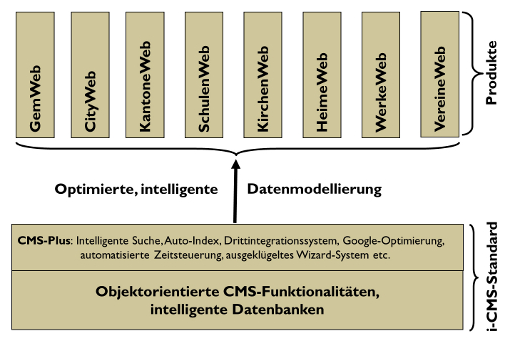
\includegraphics[width=9cm]{icms.png}
  \caption{i-CMS Modularität \parencite{iweb2019revue}}
  \label{fig: icms}
\end{figure}

Diese Modularität ermöglicht es ein breites Spektrum an Kunden zu bedienen, wobei das Angebot immer auf den Kunden zugeschnitten bleibt. Dabei liegt der Fokus der Zielgruppe auf Verwaltungen und Vereinen. Es lassen sich Module für Städte, Gemeinden sowie Kantone einbinden. Beispielsweise beim Modul KantonWeb stehen zusätzlich zu den üblichen CMS-Funktionen ebenfalls Kantonsspezifische Module, wie zum Beispiel die kantonale Rechtspflege, die eingebunden werden kann \parencite{iwebwebsiteKanotonWeb}.

I-CMS wird von einigen Gemeinde-, Stadt- und Kantonsverwaltungen eingesetzt. In der unten stehenden Grafik \ref{fig: iwebmap2019} wird veranschaulicht, in welchen Gebieten der Schweiz i-CMS überall zum Einsatz kommt. Rot markiert sind die Gemeinden, in welchen ein Webauftritt mittels i-CMS eingeführt wurde. Gemäss \parencite[S. 14]{iweb2018revue}, waren es im August 2018 über 800 Kunden, davon ungefähr 550 Gemeinde und Stadtverwaltungen \parencite{iwebwebsiteGemeindeWeb}.

\begin{figure}[h]
  \centering
  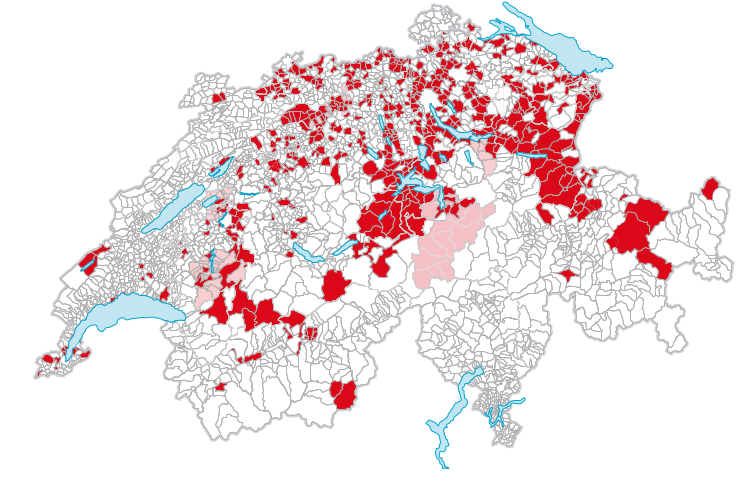
\includegraphics[width=9cm]{iweb-map-2019.png}
  \caption{i-web Marktpräsenz \parencite[S. 14]{iweb2019revue}}
  \label{fig: iwebmap2019}
\end{figure}

Wie in der Abbildung \ref{fig:icmszuwachs} ersichtlich ist, gewinnt i-CMS in den vergangen Jahren an Kunden. Dies macht i-CMS und dessen Business-Statistiktool zu einem ernstzunehmenden Konkurrenten anderer Analysetools.  

\begin{figure}[h]
  \centering
  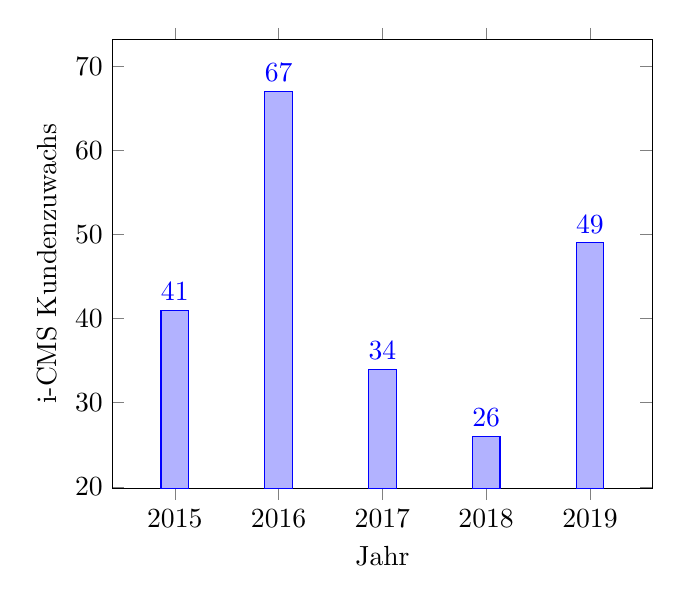
\begin{tikzpicture}  
    \begin{axis}  
    [  
        ybar,  
        enlargelimits=0.15,  
        ylabel={i-CMS Kundenzuwachs}, % the ylabel must precede a # symbol.  
        xlabel={Jahr},  
        symbolic x coords={2015, 2016, 2017, 2018, 2019}, % these are the specification of coordinates on the x-axis.  
        xtick=data,  
         nodes near coords, % this command is used to mention the y-axis points on the top of the particular bar.  
        nodes near coords align={vertical},  
        ]  
    \addplot coordinates {(2015,41) (2016,67) (2017,34) (2018,26) (2019,49)};  
    \end{axis}  
    \end{tikzpicture}  
  \caption{Kundenzuwachs i-CMS \parencite[S.7]{iweb2015revue}, \parencite[S. 7]{iweb2016revue}, \parencite[S. 7]{iweb2017revue}, \parencite[S. 14]{iweb2018revue}, \parencite[S. 14]{iweb2019revue}}
  \label{fig:icmszuwachs}
\end{figure}

\subsubsection{Funktionalitäten und Eigenschaften}
Der Hersteller von i-CMS gibt auf der Webseite keine Informationen dazu preis, welche Funktionen das Tool bietet. Jedoch sind einige Eigenschaften auf Anfrage genannt worden. Das Analysetool des i-CMS bietet gemäss Innovative Web AG (siehe Anhang \ref{appendix:emailiweb}) die Folgenden Funktionalitäten an:

\begin{quote}
  "Die integrierte Business-Statistik zeichnet die Zugriffe eindeutiger Benutzer/-innen pro Modul auf (meistbesuchte Module und meistbesuchte Objekte pro Modul).. Auch detaillierte Informationen zum Benutzerverhalten (Herkunft, Suchbegriffe, Nutzung eGov-Applikationen usw.) werden aufgezeichnet. Dazu kommen Informationen zur Infrastruktur (Geräte und Betriebssysteme), Loyalität (Aufenthaltsdauer, Anzahl besuchte Seiten) usw."
\end{quote}

Verwaltungen die i-CMS einsetzen, bewerten die Funktionen des integrierten Analysetools wie dies in Tabelle \ref{tab: icmsfeaturebewertung} dargestellt ist. 

\begin{table}[h]
	\centering
	\begin{tabular}{ | p{4cm} | p{10cm} |}
		\hline
    \textbf{Eigenschaften} & \textbf{Bewertung}  \\
    \hline 
    \multicolumn{2}{|c|}{\textit{Service}}\\ \hline 
    Affordability  &  kann nicht beantwortet werden \\ \hline
    Supportability & mangelhaft \\ \hline
    Service-Integration & kann nicht beantwortet werden \\ \hline
    Changeability  & kann nicht beantwortet werden \\ \hline
    \multicolumn{2}{|c|}{\textit{Zugänglichkeit}}\\ \hline 
    Understandability   & in Ordnung \\ \hline
    Documentation  & gut \\ \hline
    Installability & in Ordnung \\ \hline
    Learnability  & in Ordnung \\ \hline
    Accessibility  & ausgezeichnet \\ \hline
    \multicolumn{2}{|c|}{\textit{Datensicherheit}}\\ \hline 
    Datenschutz  & in Ordnung \\ \hline
    Datenhoheit & ausgezeichnet \\ \hline
    Datenzugriff  & gut \\ \hline
    Identity  & kann nicht beantwortet werden \\  \hline
    Community  & mangelhaft \\ \hline
    \multicolumn{2}{|c|}{\textit{Datenverarbeitung}}\\ \hline 
    Datenerfassung  & gut \\  \hline
    Datenvisualisierung & gut \\ \hline
    Datenanalyse & gut \\ \hline
    Datenvolumen & gut \\ \hline
    Datenaktualität  & gut \\ \hline
	\end{tabular}
	\caption{i-CMS Webanalysetool - Durchschnittliche Bewertung der Eigenschaften \parencite{softwareProcurementEvaluationTable}, \parencite[S. 178]{nakatani2011toolselectionmethod} gemäss Umfrage (siehe Anhang \ref{appendix:umfrage})}
	\label{tab: icmsfeaturebewertung}
\end{table}

\subsubsection{Datenschutz}
Innovative Web AG gibt auf ihrer Webseite \parencite{iwebwebsiteKanotonWeb} an, dass i-CMS und sämtliche Erweiterungsmodule Datenschutz konform sind. Dies wird dadurch erreicht, dass alle Webseiten die das i-CMS verwenden eine Einwilligung durch den Benutzer erfordern, die Datenschutzbestimmungen zu akzeptieren. Wie auf der Abbildung \ref{fig: urweb} zu sehen ist, geschieht die Einwilligung durch einen Knopfdruck auf "Ja" zu der Frage: "Dürfen wir Ihre anonymisierten Daten verwenden ?". Es werden weitere Massnahmen unternommen, die Daten der Benutzer so gut wie möglich zu schützen.

\begin{figure}[h]
  \centering
  
\includegraphics[width=15cm]{ur-website.png}
  \caption{Webseite des Kanton Uri \parencite{webseiteKantonUri}}
  \label{fig: urweb}
\end{figure}

Die Verarbeitung der Daten findet laut Innovative Web AG \parencite{iwebwebsiteCMS} ausschliesslich in der Schweiz statt (siehe auch Abbildung \ref{fig: urweb}) und werden anonymisiert gehalten. Es können aus den gesammelten Daten der Statistik also keine Rückschlüsse auf einzelne Personen gezogen werden. Dies wird durch den Hersteller bestätigt. Gemäss Innovative Web AG (siehe Anhang \ref{appendix:emailiweb}), gewährleistet das Analysetool des i-CMS den Datenschutz folgendermassen:

\begin{quote}
  "Die Datenschutzkonformität der Datensammlung wird sichergestellt durch Anonymisierung und “Einwilligungs-Knopf"
\end{quote}

\subsubsection{i-CMS - Fazit}

I-CMS zeigt sich als gutes Tool für Verwaltungen, da es durch seine Komplettlösung alle Bedürfnisse bis hin zur Webanalyse abdeckt. Auch für die Datenschutzkonformität ist gesorgt, was der Verwaltung eine grosse Erleichterung bring. Speziell für kleinere Verwaltungen, wie Gemeinde- oder Stadtverwaltungen, bietet i-CMS eine kompakte Lösung, welche die Suche nach einem Analysetool erübrigt. 

\subsection{Erwähnenswerte Tools}

Vereinzelt traten in der Umfrage (siehe Anhang \ref{appendix:umfrage}) andere, etwas unbekanntere Tools auf. Diese werden in diesem Kapitel kurz erläutert. 

\subsubsection{Ryte}

Ryte ist ein Kostenpflichtiges Webanalysetool hergestellt in Deutschland. Es bietet sowohl inhaltliche Analysen, wie auch technische Analysen wie zum Beispiel JavaScript Crawling. Es eignet sich also für Webseiten deren Quellcodeverwaltung intern gehalten wird \parencite{RyteFeatures}. Es wird auch eine Gratisversion von Ryte, Ryte Free, angeboten \parencite{RyteFree}.

Anwender von Ryte gaben an das Tool ausgewählt zu haben, da es einfache und aufschlussreiche Analysen ermöglicht (siehe Anhang \ref{appendix:umfrage}). Ausserdem wurde als Muss-Kriterium angegeben, dass das Verwenden eines Webanalysetools gratis sein müsse. Daraus lässt sich schliessen, dass in jener Verwaltung Ryte Free verwendet wird. Die Bewertung der Features fällt durchschnittlich aus, mit guten Visualisierungen und Auswertungen. Die Dokumentation und Erlernbarkeit des Tools fallen ein bisschen schwach aus. 

\subsubsection{SiteImprove}

SiteImprove Analytics bietet durch Features wie Echtzeit-Feedback und Analysen Einblicke in das Benutzererlebnis. Ausserdem werden von SiteImprove zum Analysetool hinzu noch weitere Services angeboten, wie zum Beispiel eine Qualitätskontrolle \parencite{SiteimproveFeatures}.

Laut den Anwender von SiteImprove die an der Umfrage (siehe Anhang \ref{appendix:umfrage}) beteiligt waren, zeichnet sich SiteImprove durch einen ausgezeichneten Support aus. Ausserdem werden auch die Massnahmen über den Datenschutz wertgeschätzt.


\subsection{Webanalysetools im Verwaltungskontext}

Aufgrund der Analysen im Kapitel \ref{sec:marktangebotwebanalyse} wurde ersichtlich, dass sich nicht alle Tools gleichermassen für den Einsatz im Verwaltungskontext eignen. Einige Tools, wie zum Beispiel Facebook Analytics (siehe Abschnitt \ref{subsec:FacebookAnalytics}), bieten nicht genügend Datenschutzmassnahmen um für Verwaltungen attraktiv zu sein. Sich eignende Tools sind definitiv Matomo und i-CMS. Dies bestätigt auch die Praxis: Die beiden Tools werden von Verwaltungen, wie dies in Abbildung \ref{fig:verwVerteilungTools} ersichtlich ist, am häufigsten eingesetzt. Zudem scheint auch Google Analytics, wenn auch verbunden mit aufwendigen Massnahmen zur Gewährleistung des Datenschutzes, gangbar zu sein. Zudem bietet Google durch seine überwältigende Marktpräsenz eine Vielzahl an Ressourcen, und gilt zu einem gewissen Grad als der Standard der Webanalyse. Die drei Tools, Google Analytics, Matomo, und i-CMS wurden ausgewählt, um eine Toolauswahl zu simulieren. Dies wird in Kapitel \ref{sec:toolsel}

\section{Vorgehen bei der Tool-Auswahl} \label{sec:toolsel}

Durch die gesetzlichen Gegebenheiten und Anforderungen an Analysetools im Verwaltungskontext, ist die Auswahl eines Tools stark daran gebunden, was das jeweilige Tool für Möglichkeiten vorweist, datenschutzgerecht Tracking zu betreiben. Da dies aber sowohl von dem Einsatzgebiet der Verwaltung, als auch dem jeweiligen Tool abhängig ist, kann keine definitive Aussage gemacht werden, welches Tool sich am besten eignet. Zudem kommen nebst dem Datenschutz auch andere Kriterien hinzu, die nicht vernachlässigt werden sollten. Schlussendlich muss das Tool auch gut bedienbar und benutzerfreundlich sein, um im Produktionseinsatz Anklang zu finden. Dementsprechend muss jede Verwaltung separat analysieren können, welches Tool sich am besten eignet. Wie eine solche Analyse aussehen könnte, wird in diesem Kapitel erläutert. 

\subsection{Tool Auswahl nach AHP} \label{subsec:toolauswAHP}

Die Webanalysetool-Auswahlmethode von Nakatani \textit{et al.} \parencite{nakatani2011toolselectionmethod} verwendet einen Ansatz basierend auf der AHP-Methode (Analytic Hierarchy Process) zur Entscheidungshilfe. AHP ist eine weitverbreitete Methode und wird in diversen Felder angewendet und eignet sich zur Selektion eines Webanalysetools für alle Arten von Organisationen \parencite[S. 176]{nakatani2011toolselectionmethod}. 

Als Entscheidungsziel gilt "Das optimale Webanalysetool für die Webseite unserer Verwaltung finden."

Die Alternativen entsprechen GoogleAnalytics, Matomo, und i-CMS von Innovative Web AG. Diese Eingrenzung wurde aufgrund der Erkenntnisse im Kapitel \ref{sec:marktangebotwebanalyse} gemacht. 

\newpage
Für die verwendeten Kriterien wurde im Kapitel \ref{sec:marktangebotwebanalyse} die Grundlage gelegt. Als Kriterien und deren Subkriterien gelten. Die Abkürzungen dienen der vereinfachten Darstellung in den Matrizen:

\begin{itemize}
  \item Service \textbf{(Service)} \begin{itemize}
    \item Affordability  \textbf{(Afford.)}
    \item Supportability \textbf{(Support.)}
    \item Service-Integration \textbf{(Service.)}
    \item Changeability \textbf{(Change.)}
  \end{itemize}
  \item Zugänglichkeit \textbf{(Zugängl.)} \begin{itemize}
    \item Understandability
    \item Documentation
    \item Installability
    \item Learnability
    \item Accessibility
  \end{itemize}
  \item Datensicherheit \textbf{(Datensich.)} \begin{itemize}
    \item Datenschutz
    \item Datenhoheit
    \item Datenzugriff
    \item Identity
    \item Community
  \end{itemize}
  \item Datenverarbeitung \textbf{(Datenver.)} \begin{itemize}
    \item Datenerfassung
    \item Datenvisualisierung
    \item Datenanalyse
    \item Datenvolumen
    \item Datenaktualität
  \end{itemize}
\end{itemize}
\newpage

Da sich die Wichtigkeit der Kriterien von Organisation zu Organisation unterscheiden, werden für die nachfolgenden Berechnungsbeispiele der Kriterien Schauzahlen verwendet. Die Zahlen der Gegenüberstellung der Tools leitet sich aus den Ergebnissen der Umfrage (siehe Anhang \ref{appendix:umfrage}) ab. Zur Umrechnung der Ergebnisse auf die Werte zur Verwendung in AHP wurde die Umrechnungsmatrix veranschaulicht in Tabelle \ref{tab:umrechMatrix} verwendet. Punktzahlen für nicht beantwortbare Kriterien wurden im Ermessen des Autors vergeben:

\begin{table}[h]
	\centering
  \begin{tabular}{cccccc}
    & nicht beantw. & mangelhaft & i.O & gut & ausgezeichnet \\
    nicht beantw. & 1 & 0,25 - 0,5 & 0,25 - 0,5 & 0,25 - 0,5 & 0,25 - 0,5 \\
    mangelhaft & 2-4 & 1 & 0,5 & 0,333 & 0,25 \\
    in Ordnung & 2-4 & 2 & 1 & 0,5 & 0,333 \\
    gut & 2-4 & 3 & 2 & 1 & 0,5 \\
    ausgezeichnet & 2-4 & 4 & 3 & 2 & 1 \\
    \end{tabular} 
	\caption{Umrechnugsmatrix - Umfrageergebnisse zu AHP Punktzahl}
	\label{tab:umrechMatrix}
\end{table}

Für die Hauptkriterien können nun mittels der Matrix in Tabelle \ref{tab:MatrixHauptkriterien} die Gewichtungen ermittelt werden. Die Gewichte der Hauptkriterien dienen der Verrechnung mit den Unterkriterien: 

\begin{table}[h]
	\centering
\begin{tabular}{ccccc}
  & Service & Zugängl. & Datensich. & Datenver. \\
  Service & 1 & 2 & 0,5 & 2 \\
  Zugängl. & 0,5 & 1 & 0,5 & 2 \\
  Datensich. & 2 & 2 & 1 & 2 \\
  Datenver. & 0,5 & 0,5 & 0,5 & 1 \\
  Summe & 4 & 5,5 & 2,5 & 7 \\
  \end{tabular} 
	\caption{ Matrix der Hauptkriterien (AHP)}
	\label{tab:MatrixHauptkriterien}
\end{table}

Normalisiert sieht die Matrix aus wie dies in Tabelle \ref{tab:MatrixHauptkriterienGewicht} Die Hauptkriterien haben das Gewicht G: 
\begin{table}[h]
	\centering
\begin{tabular}{cccccc}
  & Service & Zugängl. & Datensich. & Datenver. & G \\
  Service & 0,250 & 0,364 & 0,200 & 0,286 & 0,275 \\
  Zugängl. & 0,125 & 0,182 & 0,200 & 0,286 & 0,198 \\
  Datensich. & 0,500 & 0,364 & 0,400 & 0,286 & 0,387 \\
  Datenver. & 0,125 & 0,091 & 0,200 & 0,143 & 0,140 \\
  \end{tabular} 
  \caption{Normalisierte Matrix der Hauptkriterien mit Gewichtungen (AHP)}
\label{tab:MatrixHauptkriterienGewicht}
\end{table}	

Gleichermassen, können nun die Matrizen für die Subkriterien erstellt werden. Anhand der Subkriterien des Hauptkriterium Service, wird dies in Tabelle \ref{tab:Matrixsubkritserv} und Tabelle \ref{tab:MatrixsubkritservNorm} veranschaulicht ist. Für die Berechnungen der restlichen Kriterien siehe Anhang \ref{appendix:berechnungAHP}:

\begin{table}[h]
	\centering
\begin{tabular}{ccccc}
  & Afford. & Support. & Service. & Change. \\
  Afford. & 1 & 2 & 3 & 3 \\
  Support. & 0,5 & 1 & 2 & 2 \\
  Service. & 0,33 & 0,5 & 1 & 1 \\
  Change. & 0,33 & 0,5 & 1 & 1 \\
  Summe & 2,17 & 4 & 7 & 7 \\
\end{tabular} 
\caption{Matrix der Service-Subkriterien mit Gewichtungen (AHP)}
\label{tab:Matrixsubkritserv}
\end{table}

Die Subkriterien erhalten zudem ein relatives Gewicht. Das relative Gewicht rG berechnet sich aus dem Gewicht G des Hauptkriteriums, im Falle des Service-Kriteriums 0,275, multipliziert mit dem Gewicht des jeweiligen Subkriteriums. Dies ist in der Tabelle \ref{tab:MatrixsubkritservNorm} dargestellt:

\begin{table}[h]
  \centering
  \begin{tabular}{ccccccc}
    & Afford. & Support. & Service. & Change. & G & rG \\
    Afford. & 0,462 & 0,500 & 0,429 & 0,429 & 0,455 & 0,125 \\
    Support. & 0,231 & 0,250 & 0,286 & 0,286 & 0,263 & 0,072 \\
    Service. & 0,154 & 0,125 & 0,143 & 0,143 & 0,141 & 0,039 \\
    Change. & 0,154 & 0,125 & 0,143 & 0,143 & 0,141 & 0,039 \\
    \end{tabular} 
  \caption{Normalisierte Matrix der Service-Subkriterien mit relativem Gewicht (AHP)}
  \label{tab:MatrixsubkritservNorm}
  \end{table}

  Die Gegenüberstellung der Tools für das Subkriterium Affordability ist in der Tabelle \ref{tab:matrixAffordTools} dargestellt. Dies dient als Grundlage zur Ermittlung der gewichteten Punktzahl der Tools bei der Erfüllung eines Kriteriums:

  \begin{table}[h]
    \centering
    \begin{tabular}{cccc}
      \textbf{Affordability} & Google Analytics & Matomo & i-CMS \\
      Google Analytics & 1 & 0,5 & 3 \\
      Matomo & 2 & 1 & 2 \\
      i-CMS & 0,33 & 0,5 & 1 \\
      Summe & 3,33 & 2 & 6 \\
      \end{tabular} 
    \caption{Erfüllung des Subkriteriums Affordability der Tools (AHP)}
    \label{tab:matrixAffordTools}
    \end{table}

    Aus der normalisierten Matrix kann die gewichtete Punktzahl gP für das Subkriterium Affordability abgeleitet werden. Dies ist in Tabelle \ref{tab:matrixAffordNormalized} ersichtlich:

    \begin{table}[h]
      \centering
      \begin{tabular}{ccccc}
        \textbf{Affordability} & Google Analytics & Matomo & i-CMS & gP \\
        Google Analytics & 0,300 & 0,250 & 0,500 & 0,350 \\
        Matomo & 0,600 & 0,500 & 0,333 & 0,478 \\
        i-CMS & 0,100 & 0,250 & 0,167 & 0,172 \\
        \end{tabular} 
      \caption{Normalisierte Matrix mit gewichteter Punktzahl des Subkriteriums Affordability (AHP)}
      \label{tab:matrixAffordNormalized}
      \end{table}

      \newpage
      Abschliessend können nun die gewichteten Punktzahlen mit dem relativen Gewicht multipliziert werden. Durch das zusammenzählen der Resultate ergibt sich die Gesamtpunktzahl für jedes Tool. Dies zeigt Tabelle \ref{tab:gewPunkt}:
      \begin{table}[h]
        \centering
        \begin{tabular}{cccc}
          & Google Analytics & Matomo & i-CMS \\
          Affordability & 0,044 & 0,060 & 0,022 \\
          Supportability & 0,039 & 0,014 & 0,019 \\
          Service-Integration & 0,017 & 0,011 & 0,010 \\
          Changeability & 0,007 & 0,025 & 0,007 \\
          Understandability & 0,012 & 0,025 & 0,012 \\
          Documentation & 0,022 & 0,011 & 0,022 \\
          Installability & 0,011 & 0,021 & 0,005 \\
          Learnability & 0,010 & 0,010 & 0,010 \\
          Accessibility & 0,005 & 0,010 & 0,010 \\
          Datenschutz & 0,020 & 0,099 & 0,063 \\
          Datenhoheit & 0,010 & 0,041 & 0,041 \\
          Datenzugriff & 0,012 & 0,012 & 0,012 \\
          Identity & 0,006 & 0,023 & 0,007 \\
          Community & 0,017 & 0,017 & 0,006 \\
          Datenerfassung & 0,008 & 0,008 & 0,016 \\
          Datenvisualisierung & 0,013 & 0,007 & 0,007 \\
          Datenanalyse & 0,011 & 0,011 & 0,011 \\
          Datenvolumen & 0,012 & 0,006 & 0,006 \\
          Datenaktualität & 0,003 & 0,014 & 0,007 \\
          \textbf{Gewichtete Punktzahl} & \textbf{0,281} & \textbf{0,425} & \textbf{0,294} \\
          \end{tabular} 
        \caption{Gesamtpunktzahl der Tools (AHP)}
        \label{tab:gewPunkt}
        \end{table}


        \subsection{Empfehlung bei der Toolauswahl}
        Die Berechnung in Kapitel \ref{subsec:toolauswAHP} ergibt das Resultat, dass Matomo sich unter den kreierten Bedingungen (siehe Anhang \ref{appendix:berechnungAHP}) am besten eignen würde. Dieses Resultat kann, abhängig davon wie die einzelnen Verwaltungen oder Organisationen die Wichtigkeit der Kriterien und Subkriterien bewerten, andere Werte annehmen. Mit jener Berechnung soll lediglich gezeigt werden, wie Verwaltungen Vorgehen können, um bei der Auswahl eines Tools eine Entscheidung treffen zu können. Es empfiehlt sich, eine eigene Berechnung, spezifisch für die eigene Organisation durchzuführen. Die Bewertung der Punktzahl der einzelnen Tools bei der Erfüllung der Kriterien basiert auf den Werten der Umfrage (siehe Anhang \ref{appendix:umfrage}). Diese Werte basieren auf den Meinungen einzelner Personen. Daher empfiehlt es sich, ebenfalls die Punktzahl-Werte der Tool-Vergleiche nach einer eigenen Analyse der Tools anzupassen. Um eine eigene Berechnung durchzuführen, hat der Autor eine Spreadsheet-Datei erstellt, welche die Berechnung automatisch durchführt:

        \url{https://docs.google.com/spreadsheets/d/1e5vWmMwuKuDppYaflFVkWFBMY2u9siwfa3mRG3LnEFY/copy}


        \newpage

\section{Reflexion}
Die Ziele der Arbeit, einen Überblick über Analysetools und deren Funktionen zu verschaffen und ein Vorgehen für die Auswahl eines Tools konnten erreicht werden. Jedoch waren zum Zeitpunkt des Verfassens der Arbeit durch die Pandemie des SARS-CoV-2 nicht nur der Autor, sondern jegliche Verwaltungen betroffen. Es stellte sich als schwierig heraus, durch die Umfrage an genügend Informationen zu kommen, um repräsentative Aussagen machen zu können. Speziell für die Beurteilung der Tools fehlte die Quantität der Teilnehmer, um jedes Tool aussagekräftig beschreiben zu können. Ein Grund dafür ist mitunter, dass mit der Umfrage zu spät begonnen wurde. Ein weiterer Grund ist, dass die Umfrage auf ein sehr spezifisches Publikum abgerichtet ist. Es war nicht ganz einfach, die richtige Person, den Webmaster, bei mehreren Verwaltungen ausfindig zu machen. Zusätzlich musste diese Person natürlich auch einwilligen an der Umfrage teilzunehmen. Die Webmaster der Web-Plattformen der Verwaltungen dürften jedoch auch durch die Pandemie zusätzlich ausgelastet gewesen sein. Ich hatte mir erhofft durch die Umfrage die These aussagekräftiger beantworten zu können.

Auch den Inhalt der Umfrage sinnvoll zu wählen, war nicht einfach. Es war von zu Beginn angedacht, zu erheben was für Tools im Verwaltungskontext eingesetzt werden. Es wurde eine Bewertungsmatrix für das Tool als Frage erstellt, was grundsätzlich sehr hilfreich war. Was jedoch ebenfalls nützlich gewesen wäre, wie es beim verfassen des letzten Kapitels zu erkennen gab, wäre eine zweite Matrix für die Meinungen der Webmaster zur Wichtigkeit der einzelnen Features gewesen. Nun da diese Daten nicht erhoben wurden, musste die Berechnung aufgrund von Beispiel Zahlen zur Wichtigkeit der Features durchgeführt werden. Beim nächsten Mal sollte, bevor die Umfrage durchgeführt wird, der Inhalt der Kapitel besser überlegt werden. Somit könnten auch Daten, deren Wichtigkeit sich nicht direkt aus der Zielsetzung ableiten lässt, erhoben werden.

Ich habe viel darüber gelernt, was es bedeutet, Webanalyse zu betreiben und wie diese funktioniert. Ebenfalls neu für mich, war die kantonale Rechtslage mit den Datenschutzgesetzen. Der Konflikt zwischen der dem Tracking von Internetbenutzern Datenschutz ist ein Spannendes Thema, dem auch ausserhalb des Verwaltungskontext in letzter Zeit viel Beachtung geschenkt wurde. Beispielsweise veränderte sich durch die DSGVO, wie Webanalyse, von Unternehmen die Services für EU-Staatsbürger anbieten, betrieben werden darf. In diese Thematik einzutauchen, war sehr aufregend. 

Ebenfalls spannend war es, mittels der AHP Methode einen wissenschaftlichen Weg aufzuzeigen, um ein Webanalysetool auszuwählen. Das Verstehen dieser Methode erforderte das Lesen einiger Anleitungen sowie das Schauen mehrerer YouTube-Videos. Doch es war sehr befriedigend, das Excel, spezifisch für die Auswahl der Webanalysetools, mit sämtlichen Eigenschaften und Alternativen aufzubauen und Berechnungen durchzuführen.

Was mir durch diese Arbeit klar wurde, ist dass Google ein mächtiges Monopol auf der Webanalyse hat. Über 80\% des gesamten Marktes verwendet das Analysetool von Google. Mit dieser Aufstellung, befindet sich Google in einer Position, in der sie den Grossteil des Internet-Traffic analysieren können. Was diese Sammlung von Daten genau bedeutet, ist unklar. Ich bin mir aber sicher, dass Tools wie Matomo, welche grossen Wert auf den Schutz der Personendaten legen, Google Analytics ein würdiger Rivale sind. Speziell für den Einsatz in Verwaltungen, scheint sich zumindest Matomo besser zu eignen.